\documentclass[a4paper,10pt]{article}
\usepackage[spanish]{babel}
\usepackage{amssymb}
\usepackage[utf8]{inputenc}
\usepackage[left=2.5cm,top=3.5cm,right=2.5cm,bottom=3.5cm]{geometry}
\usepackage{paralist}
\usepackage{lineno}
\usepackage{fancyvrb}
\usepackage{caption}
\usepackage{graphicx}
\usepackage{float}

\title{Diseño de Videojuegos \\ Análisis y Diseño del Motor de Movimiento }
\author{Rosa María Durante Lerate\\Pablo Recio Quijano\\Noelia Sales Montes}

\begin{document}
\maketitle


\tableofcontents

\section{Descripción del Problema}

Necesitamos modelar un motor de juego para un videojuego. Este motor será el
encargado de sostentar una gran parte de un videojuego tipo RPG, siendo el motor
de movimiento. \\
 
Antes de ver las funcionalidades que podemos realizar en este motor tenemos que
analizar las estructuras de datos que se necesitarán modelar para tener una
buena interacción entre las librerías SDL, la base de datos y los gráficos.
Describémoslas pues:

\begin{description}

\item [Animación]: Estructura que será la encargada de realizar las animaciones
  del personaje en el juego. También será la encargada de modelar las colisiones
  que se pueden realizar en una parte específica del juego. 
  Esto se obtendrá gracias a la Imagen definida como fondo y al Personaje
  principal que controla el usuario.

\item [BaseDatos]: Abstracción de la base de datos del sistema. Será el
  encargado de iniciar, modificar, acutalizar, consultar, borrar y cerrar la
  base de datos. Se encargará de suministrar datos tanto del inventario como de
  los personajes (estadísticas) y diálogos (personajes no jugables no combatibles).

\item [Diálogo]: Abstracción de la intervención de un personaje no jugable y no
  combatible con nuestro personaje principal. Éstos, a priori, sólo se dedicaran
  a administrar información al jugador, es decir, a tener un diálogo con el
  personaje principal.

\item [Imagen]: Abstracción del fondo del juego. Se compondrá en base a tiles
  ordenados de alguna forma que reconstruyan el mapa de juego. Dicha imágen
  estará compuesta por una matriz de imágenes (tiles) las cuales, cada posición
  de la matriz, tendrán características: colisionable/no colisionable, personaje
  no jugador, objeto, etc...

\item [Inventario]: Estructura para la realización de todos los aspectos de la
  interfaz, navegabilidad y compenetración con la base de datos.

\item [Objeto]: Abstracción de los objetos interactuables que puede encontrar el
  personaje en algún lugar del mapa. 

\item [Pantalla]: Abstracción del concepto de la pantalla del juego. Es aquí
  donde se modelará todas las animaciones, colisiones con el fondo del juego,
  interacción con los personajes no jugadores, muestra y navegabilidad en el
  inventario, etc...

\item [Personaje]: Abstración del concepto del personaje principal del
  juego. Esta estructura interactuará con la imágen de fondo, y se dedicará a
  realizar las consultas necesarias a la base de datos del sistema. Obtendremos
  el Sprite del personaje 

\item [Sprite]: Unidad mímina de imagen para el personaje. Es una imagen tipo
  bitmap donde se encuentran todas las instancias de movimiento que puede
  realizar el personaje. Para este tipo de dato necesitamos saber el número de
  filas, de columnas y de imágenes que contiene en total.

\item [Teclado]: Estructura que controlará los eventos que pueda producir el
  usuario con el teclado. Para ello necesitaremos de un enumerado para
  identificar el tipo de tecla con la que ha desencadenado el evento.

\item [Tile]: Unidad mínima de imagen para el fondo de juego. Es una imagen tipo
  bitmap donde se encuentran todos los objetos, estilo, etc que puede componer
  el fondo de juego (ejemplo, para un bosque el tile contendrá, por filas y
  columnas de un tamaño predeterminado, un árbol, un arbusto, parte de un rio,
  cielo, una nube, etc). Esta estructura de dato guardará el número de columnas
  y filas y de elementos que contiene en total.

\end{description}


Dicho esto, veamos las funcionalidades que modelaremos en este motor:
\begin{itemize}
\item \textbf{Movimiento del personaje:} La funcionalidad principal que debe
  tener todo videojuego es modelar el movimiento del personaje. En nuestro caso,
  el usuario obtendrá en este motor un fondo donde se desarrollará un nivel o
  donde permanecerá un tiempo en el juego. Además tendrá al personaje principal,
  el protagonista del juego, el cual será el personaje que puede mover el usuario. \\

  Este motor tiene una vista en 2-D de forma cenital, por lo que el personaje
  podrá desplazarse por el mapa de cuatro formas distintas: \textbf{arriba,
    abajo, derecha} e \textbf{izquierda}. Además hay que tener en cuenta que el
  mapa completo no estará del todo visible en la pantalla, ya que el tamaño del
  mapa será mayor que el de la pantalla, y que en algunos puntos de dicho mapa
  serán colisionables o interactuables. \\

\item \textbf{Colisiones entre objetos:} Como hemos dicho, habrá partes del mapa
  de juego en los que el personaje no podrá atravesar directamente o pisar. Para
  ello debemos de controlar dichas colisiones tanto con objetos interaccionables
  (objetos que el personaje pueda coger como un baúl o algo parecido para añadir
  a su inventario) u objeto sno interaccionables (paredes, árboles, arbustos, etc).

\item \textbf{Interacción entre objetos/personajes no jugables no combatibles:}
  Además de las colisiones tenemos que tener en cuenta que existirán objetos con
  los que el personaje podrá coger, utilizar o hablar (en el caso de los
  personajes no jugables y no combatibles) para obtener información. 

\item \textbf{Navegabilidad en el inventario:} Como es obvio, tenemos que dar al
  jugador la opción tanto de observar el mapa completo como de navegar en el
  inventario de los personajes. Hay que tener en cuenta que el inventario es
  común para los cuatro personajes y no solo para el principal. En dicho
  inventarion tendremos varias ocpiones a realizar: se observará el estado de
  todos los personajes; se observará los objetos curativos (común para el grupo
  completo), armaduras y armas que tienen equipados cada personaje y que tienen
  guardados sin usar cada uno; se prodrá guardar el estado del juego, pedir la
  salida del juego o restaurar a una copia guardada del juego.

\end{itemize}

\section{Análisis}
\subsection{Modelo de Casos de Uso}
\subsubsection{Diagrama de Casos de Uso}

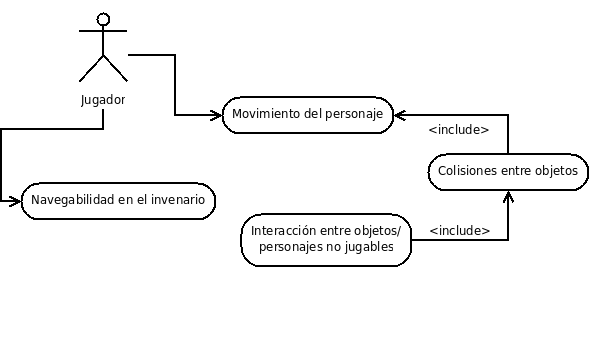
\includegraphics[scale=0.6]{Diagrama_Casos_Uso.png}

\subsubsection{Descripción de Casos de Uso}

\paragraph*{Descripción Caso de Uso: Movimiento del personaje.}
\begin{itemize}
\item \textbf{Caso de Uso:} Movimiento del personaje.
\item \textbf{Descripción:} El jugador podrá realizar cuatro tipos de
  movimientos con el personaje principal: trasladar el personaje hacia arriba,
  hacia abajo, hacia la derecha o hacia la izquierda del mapa.
\item \textbf{Actores:} Usuario o jugador del videojuego.
\item \textbf{Precondiciones:} El videojuego está iniciado y está cargado todo
  el motor de movimiento sin errores.
\item \textbf{Postcondiciones:} Ninguna.
\item \textbf{Escenario principal:} \\
\begin{enumerate}
\item El jugador pulsa la tecla 'up' del teclado.
\item El sistema mueve el personaje del juego hacia arriba del mapa.
\item El jugador colisiona con un objeto. \textbf{Include: Colisiones entre objetos.}
\end{enumerate}
\item \textbf{Escenarios alternativos o de error:} \\
\begin{itemize}
\item \textbf{1a} El jugador pulsa la tecla 'down' del teclado.
\item \textbf{  } El sistema mueve el personaje del juego hacia abajo del
  mapa.
\item \textbf{1b} El jugador pulsa la tecla 'left' del teclado.
\item \textbf{  } El sistema mueve el personaje del juego hacia la izquierda
  del mapa.
\item \textbf{1c} El jugador pulsa la tecla 'right' del teclado.
\item \textbf{  } El sistema mueve el personaje del juego hacia la derecha del
  mapa.
\item \textbf{1d} El personaje se encuentra en un borde de la pantalla y quiere
  avanzar (cualquier dirección).
\item \textbf{ 1} El sistema comprueba que existe más mapa fuera de la
  pantalla y hace que el personaje acceda a esa porción del mapa.
\item \textbf{ 2} El sistema comprueba que no existe más mapa para visualizar
  en dicha dirección y deja al personaje en la misma posición.
\end{itemize}
\end{itemize}

\paragraph*{Descripción Caso de Uso: Colisiones entre objetos.}
\begin{itemize}
\item \textbf{Caso de Uso:} Colisiones entre objetos.
\item \textbf{Descripción:} Este caso de uso tiene efecto cuando nuestro
  personaje realiza un movimiento en el mapa y, aunque no sea algún borde en el
  mapa, no es capaz de atravesarlo ya que lo que ha ocurrido es una colisión con
  un objeto 'específico' en el sistema el cual podría ser interactuable o no.
\item \textbf{Actores:} El personaje del juego dirigido por el usuario.
\item \textbf{Precondiciones:} El sistema ha cargado satisfactoriamente el motor
  y el personaje puede moverse libremente por el mapa.
\item \textbf{Postcondiciones:} Ninguna.
\item \textbf{Escenario principal:} \\
\begin{enumerate}
\item El usuario realiza un movimiento (cualquier dirección) en el mapa.
\item El sistema comprueba que no existe colisión y realiza el movimiento.
\end{enumerate}
\item \textbf{Escenarios alternativos o de error:} \\
\begin{itemize}
\item \textbf{2a} El sistema comprueba que existe una colisión en relación al
  movimiento efectuado. 
\item \textbf{ 1} El personaje permanece en la misma posición.
\item \textbf{ 2} El objeto o personaje no jugable con el que se ha realizado
  la colisión es interactuable y se acciona la acción a seguir, por ejemplo, si
  fuese un objeto lo tomará y mostrará qué objeto ha cogido o, por el
  contrario, si fuese un personaje no jugable dialogarán o
  lucharán. \textbf{Include Interacción entre objetos/pnj}.
\end{itemize}
\end{itemize}


\paragraph*{Descripción Caso de Uso: Interacción entre objetos/personajes no jugables.}
\begin{itemize}
\item \textbf{Caso de Uso:} Interacción entre objetos/personajes no jugables.
\item \textbf{Descripción:} Cuando el personaje realice una colisión al
  efectuar un movimiento con un objeto interactuable se activará la acción del
  objeto o npj.
\item \textbf{Actores:} El usuario a través del personaje del videojuego.
\item \textbf{Precondiciones:} El personaje ha realizado un movimiento.
\item \textbf{Postcondiciones:}
\item \textbf{Escenario principal:} \\
\begin{enumerate}
\item El usuario efectua la colisión con un objeto interactuable.
\item El sistema comprueba que tipo de colisión es y con qué tipo de
  objeto. Informa al usuario que el personaje ha tomado ese objeto y que se
  encuentra en el inventario (por ejemplo).
\end{enumerate}
\item \textbf{Escenarios alternativos o de error:} \\
\begin{itemize}
\item \textbf{1a} El usuario efectua la colisión con un personaje no jugable.
\item \textbf{  } El sistema comienza el diálogo asigando a ese personaje no jugable.
\end{itemize}
\end{itemize}

\paragraph*{Descripción Caso de Uso: Navegabilidad en el inventario.}
\begin{itemize}
\item \textbf{Caso de Uso:} Navegabilidad en el inventario.
\item \textbf{Descripción:} Cuando el usuario pulse en una determinada tecla
  aparecerá en la pantalla de juego el inventario de los personajes principales.
\item \textbf{Actores:} El usuario
\item \textbf{Precondiciones:} El motor de movimiento debe estar cargado en el
  sistema satisfactoriamente.
\item \textbf{Postcondiciones:} Ninguna.
\item \textbf{Escenario principal:} \\
\begin{enumerate}
\item El usuario abre el inventario.
\item El sistema muestra la pantalla principal del inventario: Los cuatro
  personajes del juego con sus características de vida y nivel. Además el
  entorno estará guiado por pestañas donde el usuario puede acceder para ver los
  objetos que tiene (curativos, armadura, etc), o para guardar/salir.
\item El usuario se desplaza de pestaña en el inventario.
\item El sistema le muestra el contenido de la pestaña a la que se desplaza.
\end{enumerate}
\end{itemize}


\subsection{Modelo Conceptual de Datos}

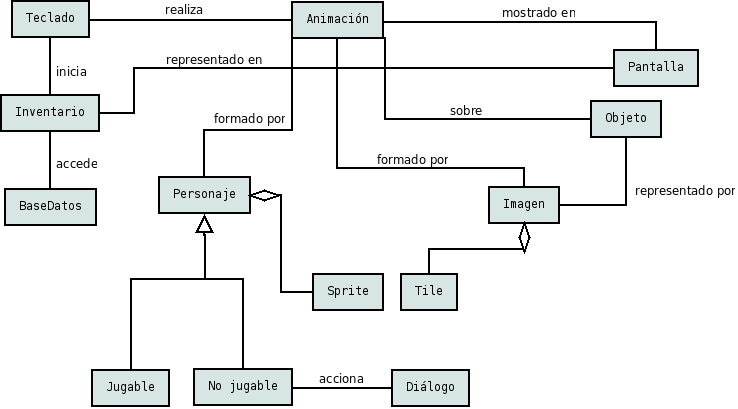
\includegraphics[scale=0.6]{Diagrama_conceptual.png}


\end{document}
